%% Paper 15 — Polymorphisms, DDI, Inhibitors figure captions

\begin{figure}[!htbp]\centering
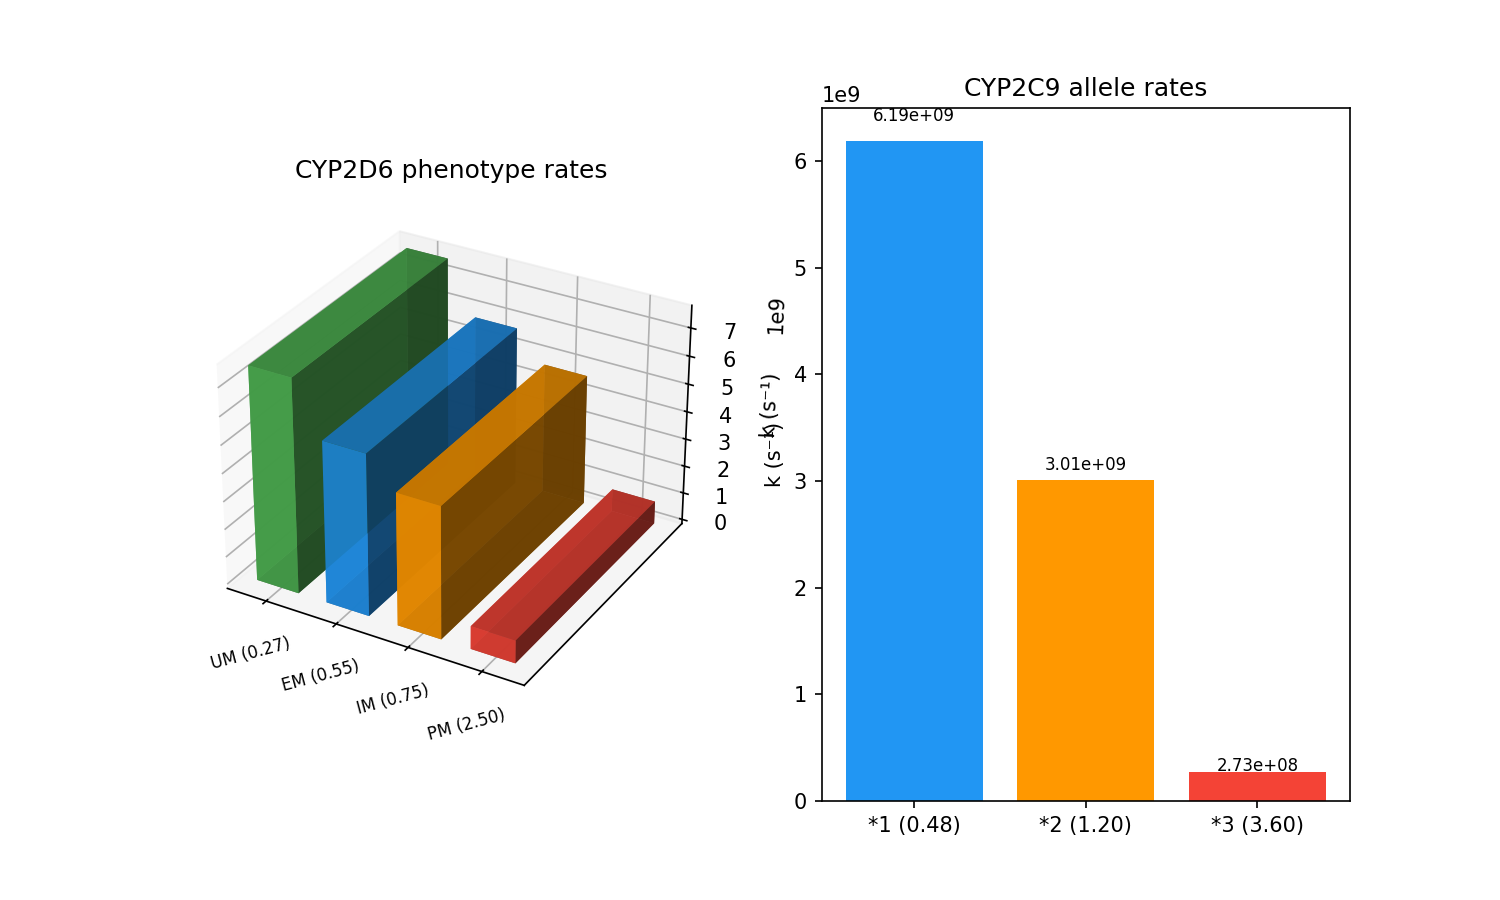
\includegraphics[width=\textwidth]{figures/panel_01_allele_dm_rates.png}
\caption{CYP2D6 phenotype rate constants from $\Delta M$ values (3D bars, left)
and CYP2C9 allele rates (right).  UM/EM/IM/PM span a 7-fold range;
CYP2C9*3 retains $<5$\,\% of wild-type activity.}\label{fig:allele}
\end{figure}

\begin{figure}[!htbp]\centering
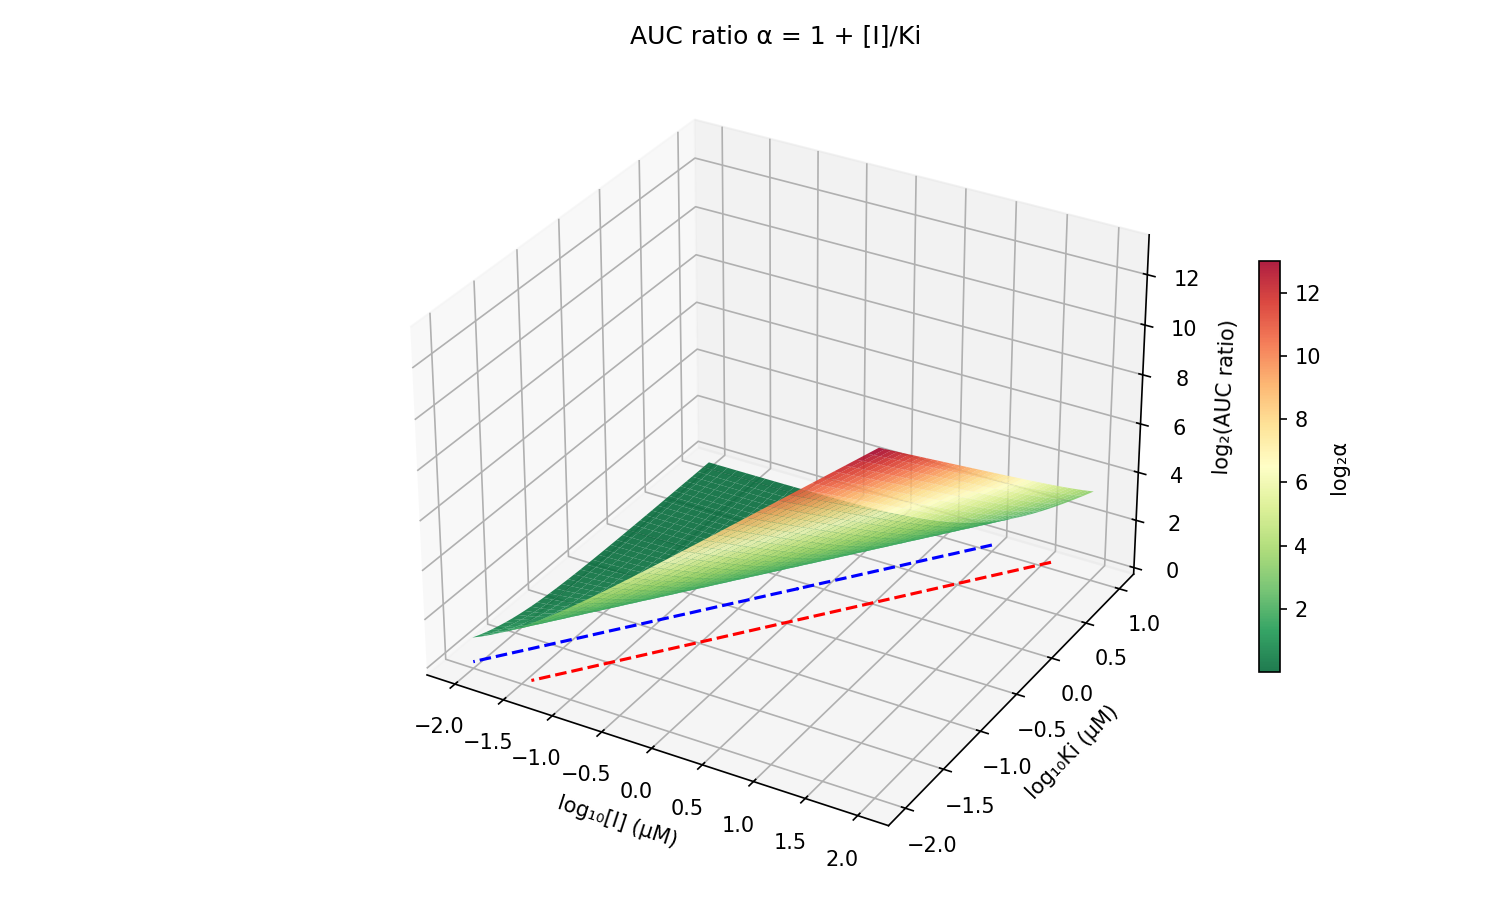
\includegraphics[width=\textwidth]{figures/panel_02_alpha_ddi_surface.png}
\caption{3D surface of AUC ratio $\alpha = 1 + [I]/K_i$ over inhibitor
concentration and $K_i$.  Contours mark the moderate (2×) and strong (5×)
DDI thresholds.}\label{fig:alpha}
\end{figure}

\begin{figure}[!htbp]\centering
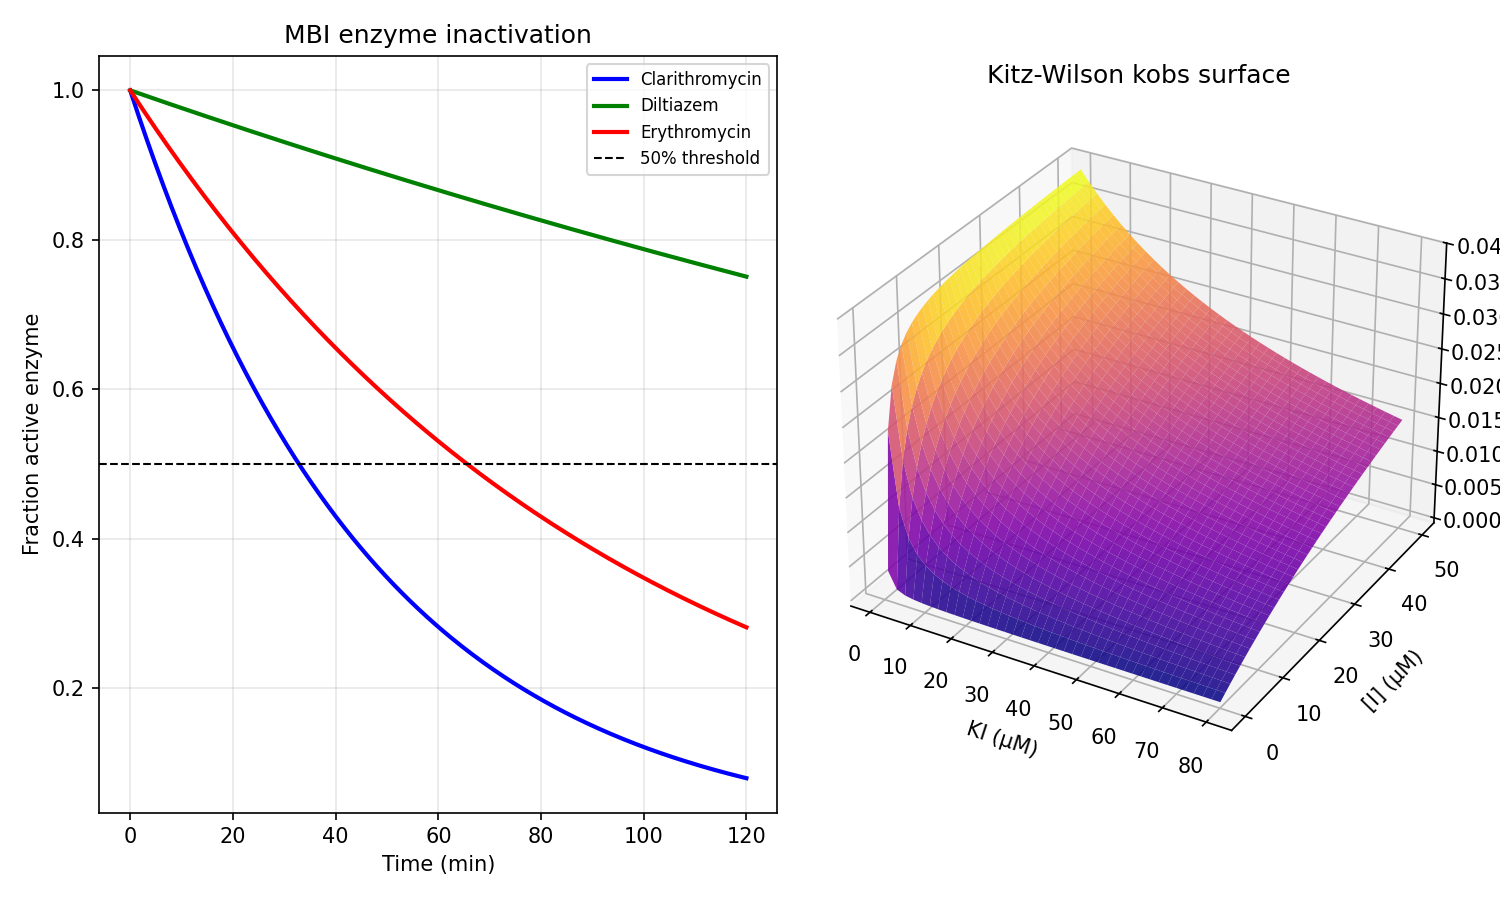
\includegraphics[width=\textwidth]{figures/panel_03_mbi_kinetics.png}
\caption{MBI enzyme inactivation curves $E(t)/E_0$ for clarithromycin,
diltiazem, and erythromycin at clinical concentrations.  Right:
Kitz--Wilson $k_\text{obs}$ surface over $K_I$ and $[I]$.}\label{fig:mbi}
\end{figure}

\begin{figure}[!htbp]\centering
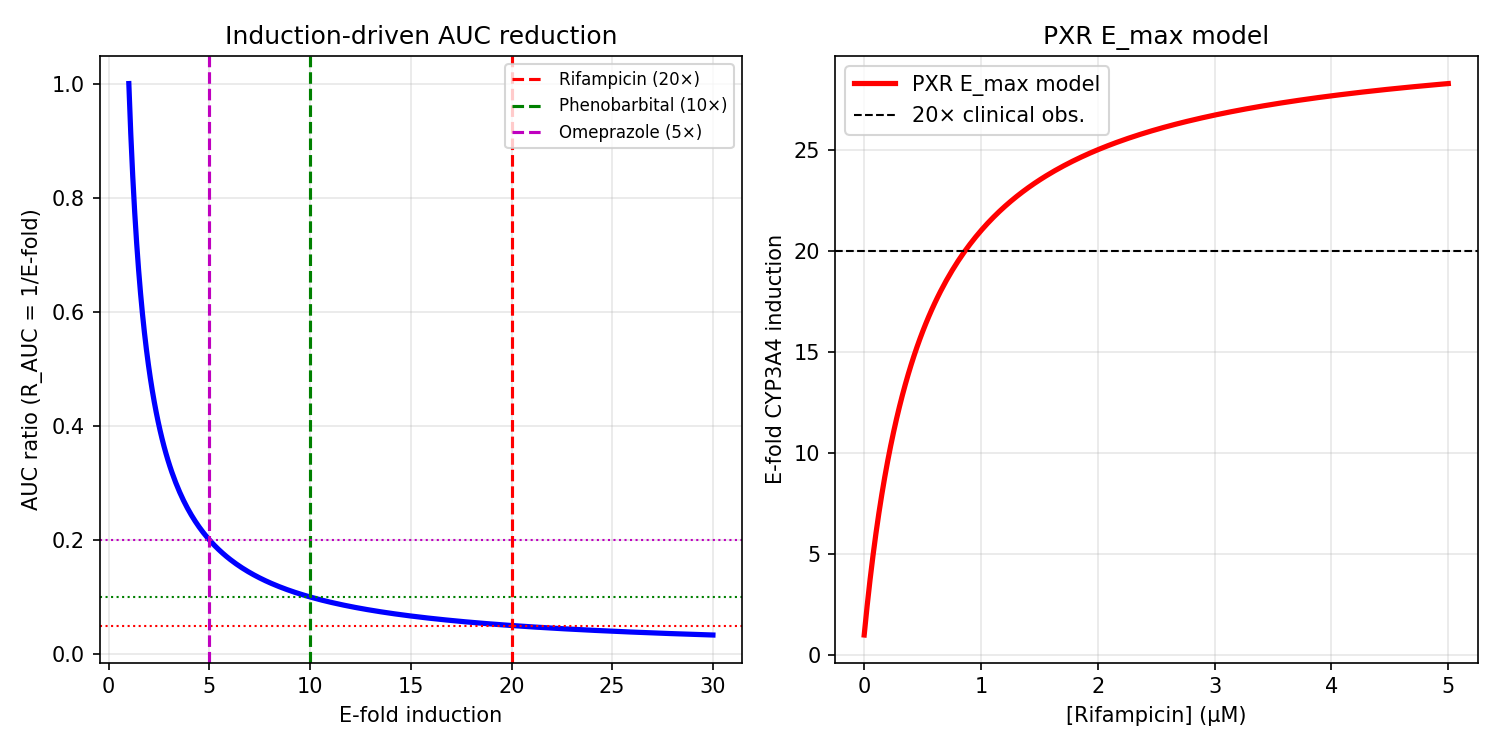
\includegraphics[width=\textwidth]{figures/panel_04_induction_auc.png}
\caption{Left: victim drug AUC ratio $R_\text{AUC} = 1/E_\text{fold}$ vs.\
fold-induction for rifampicin, phenobarbital, and omeprazole.  Right:
PXR $E_\text{max}$ model for rifampicin predicts $\approx 24$-fold induction
at 2\,$\mu$M.}\label{fig:induction}
\end{figure}

\begin{figure}[!htbp]\centering
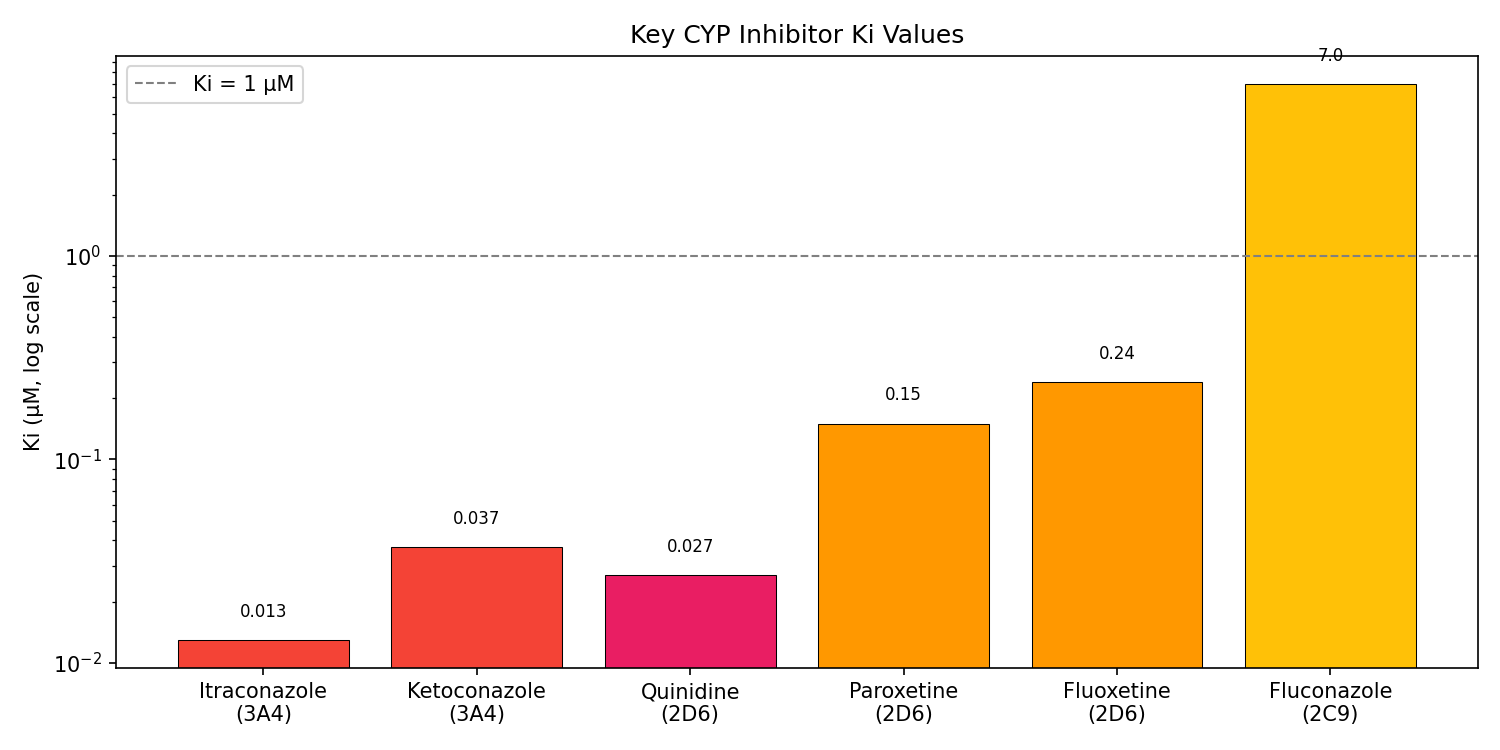
\includegraphics[width=\textwidth]{figures/panel_05_inhibitor_atlas.png}
\caption{$K_i$ values (log scale) for key CYP inhibitors across CYP3A4,
CYP2D6, and CYP2C9.  Itraconazole and quinidine have the lowest $K_i$
values ($<0.03$\,$\mu$M); fluconazole is the weakest (7\,$\mu$M on 2C9).}\label{fig:atlas}
\end{figure}

\begin{figure}[!htbp]\centering
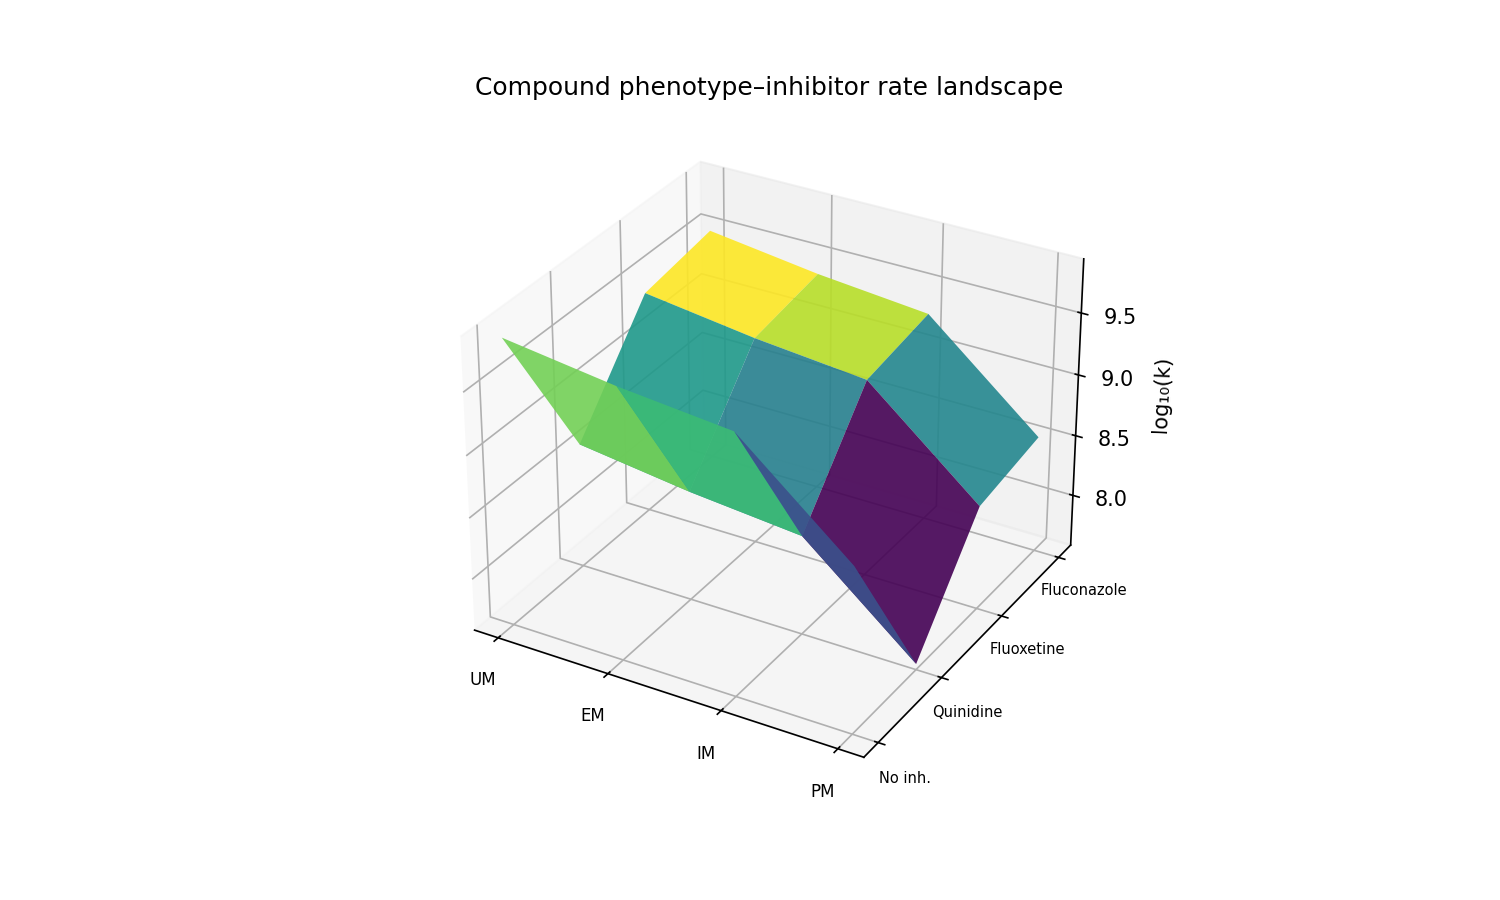
\includegraphics[width=\textwidth]{figures/panel_06_compound_phenotype.png}
\caption{3D rate landscape: $\log_{10} k$ as a function of CYP2D6 phenotype
and co-administered inhibitor.  The EM + quinidine combination produces rates
below the PM floor.}\label{fig:compound}
\end{figure}

\begin{figure}[!htbp]\centering
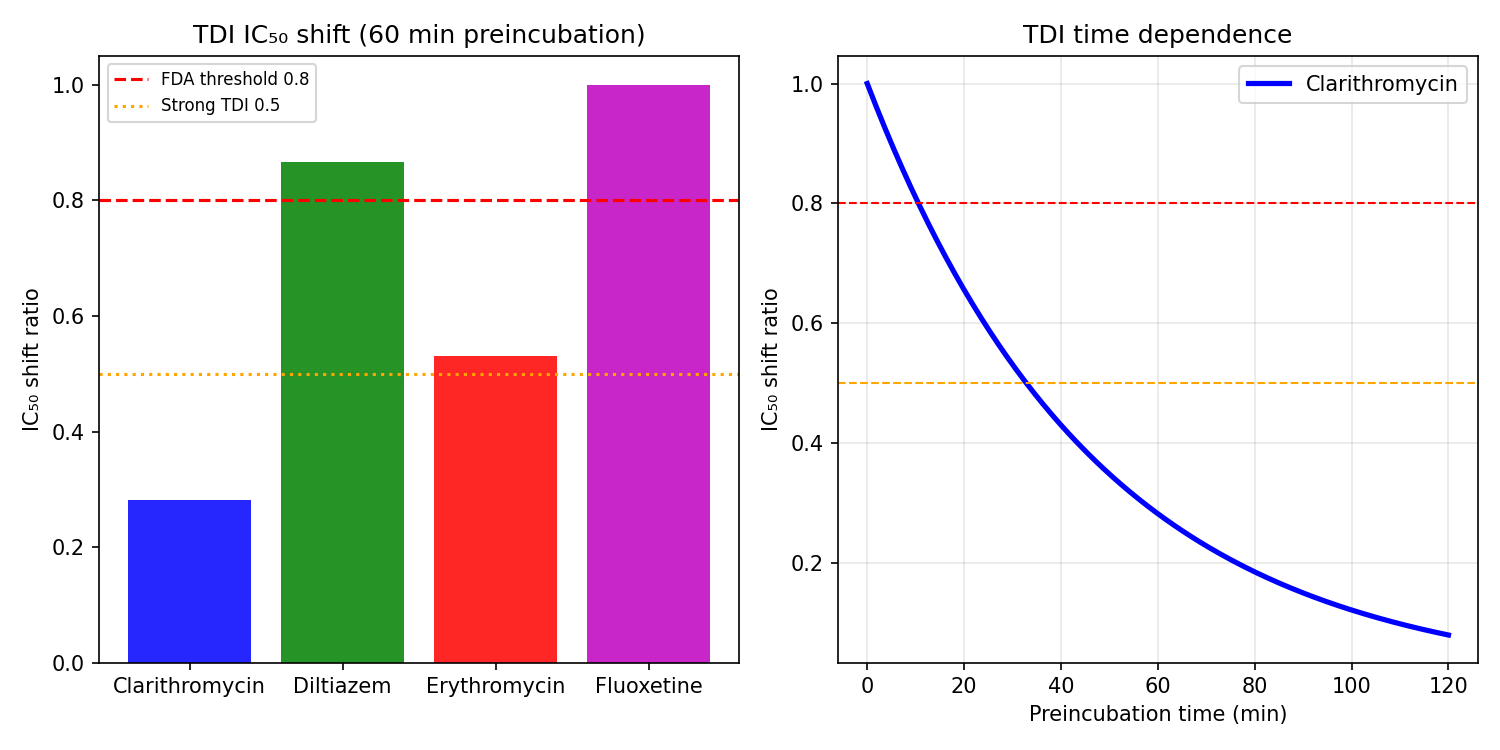
\includegraphics[width=\textwidth]{figures/panel_07_tdi_shift.png}
\caption{Left: TDI IC$_{50}$ shift ratios at 60-min preincubation.
Clarithromycin ($r = 0.28$) exceeds the strong TDI threshold; fluoxetine
($r \approx 1.0$) is non-TDI.  Right: shift ratio vs.\ preincubation time
for clarithromycin.}\label{fig:tdi}
\end{figure}

\begin{figure}[!htbp]\centering

\includegraphics[width=\textwidth]{figures/panel_08_validation.png}
\caption{Validation summary: all 8 scripts PASS for Paper~15.}\label{fig:val}
\end{figure}
